\documentclass[a4paper, 11pt]{article}
\usepackage[utf8]{inputenc}
\usepackage{graphicx}
\usepackage{fancyvrb} 
\usepackage{siunitx}
\usepackage[table, xcdraw, svgnames]{xcolor}
\usepackage{listings, lstautogobble}
\usepackage{subfig}

\renewcommand{\figurename}{Figuur}

\setlength{\parskip}{0.5em}

\title{Sensornetwerk Proof of Concept v0.2}
\author{Groep 5}
\date{September 2018}
\pagenumbering{gobble}

\begin{document}

\maketitle
\clearpage
\pagenumbering{arabic}
\clearpage

\section{Inleiding}
Dit document beschrijft de software implementaties van groep 5 voor het vak "Sensornetwerk Ontwerp" aan de Hogeschool van Amsterdam.

Het doel van de opdracht is om een dynamisch netwerk van sensornodes te maken, waarbij in dit document de nadruk ligt op de algemene netwerkstructuur en de implementatie in MCU van de sensornodes. Hiervoor geldt over het algemeen dat het stuk software wat in dit document beschreven wordt gelijk is voor alle sensornodes. Tijdens de ontwikkeling van de individuele sensorimplementaties (vak "Sensormodule Ontwerp") kan de code afhankelijk per node worden aangepast. 

Het doel van dit document is om een 'proof of concept' te geven van de algemene netwerkstuctuur waar de sensornodes tijdens het vak "Sensormodule Ontwerp" gebruik van zullen maken.


\section{Algemene Node Programma}
Zoals besproken in de inleiding van dit document het grootste deel van de programma code voor de node MCU's gelijk. In dit hoofdstuk wordt deze code besproken. 

\subsection{Routing}
Het is belangrijk dat het sensornetwerk dynamisch is. Dit wil zeggen dat het het netwerk waarover de sensordata verstuurd wordt op ieder willekeurig moment kan veranderen. In de praktijk gebeurd dit wanneer de draadloze sensornodes van plaats veranderen of uit gaan. 

Om een 'up to date' beeld te houden van de beschikbare nodes in het netwerk houdt iedere een een routing tabel bij. Deze tabel wordt opgesteld uit berichten die ontvangen worden van de directe buren van de node. In die berichten staat informatie over de directe buren van de nodes die de berichten sturen. 

%%%%%Moet nog aangevuld worden (Zie GLO)%%%%%%%
\subsection{Flowchart}
Om de algemene node-code inzichtelijk te maken is gebruik gemaakt van ene flowchart. In Figuur~\ref{fig:flowchart} is deze flowchart te zien.

\begin{figure}[!h]
	\centering	
	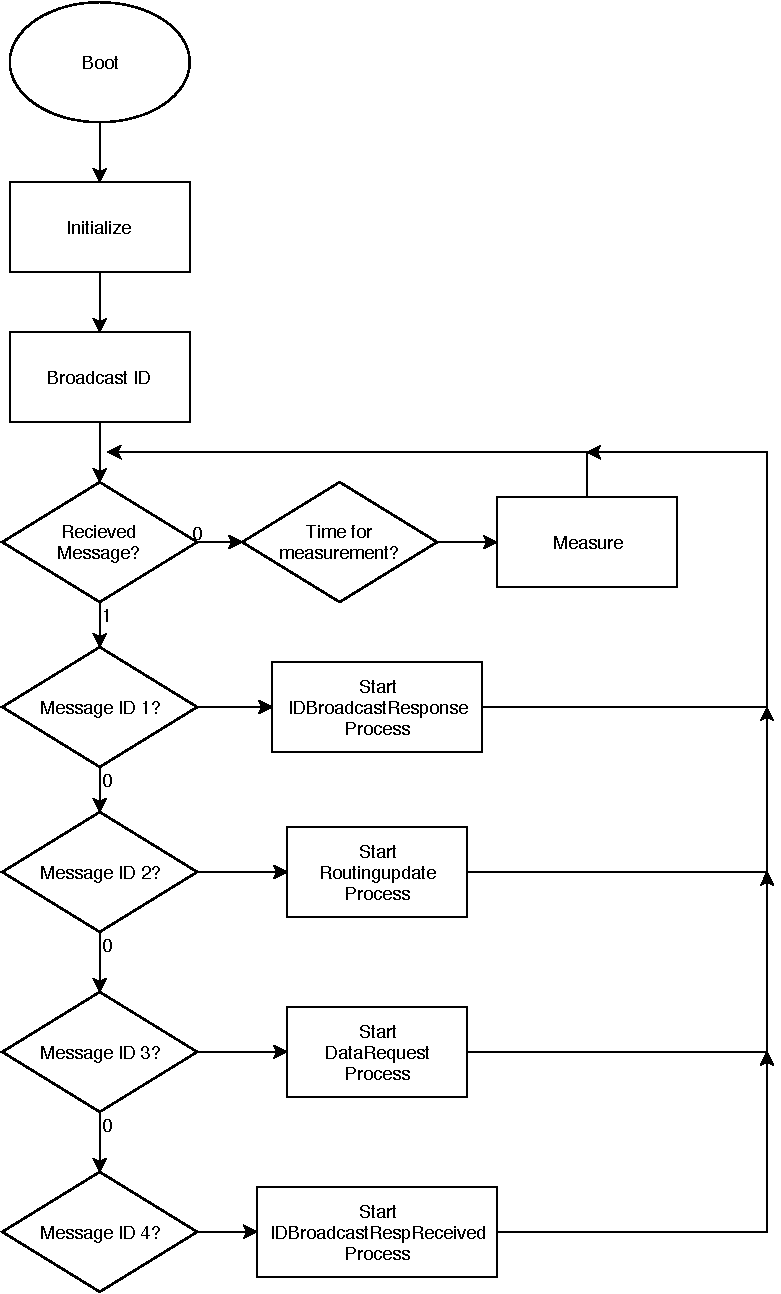
\includegraphics[width=.5\textwidth, keepaspectratio]{media/Pflow.pdf}
    \caption{Nadat de node opgestart wordt (Boot) de MCU geïnitialiseerd in het blok [Initialize]
     \textbf{Figuur dient in deze versie als voorbeeld en zal geupdate worden wanneer het basis ontwerp af is.}}
    \label{fig:flowchart}
\end{figure}
%Zie GLO

\subsection{Statemachine}
Omdat MCU veel aan het wachten is op berichten om deze vervolgens te verwerken is gekozen als implementatie een statemachine te gebruiken. Deze is afgebeeld in Figuur~\ref{fig:Statemachine} 
Statemachine die de verschillende states laat zien waar de Xmega in komt vanaf het opstarten.

\begin{figure}[!ht]
	\includegraphics[width=.8\textwidth, keepaspectratio]{media/Pstate.pdf}
    \caption{ \textbf{Figuur dient in deze versie als voorbeeld en zal geupdate worden wanneer het basis ontwerp af is.}}
    \label{fig:Statemachine}
\end{figure}
%Zie GLO

\section{Basisstation}

\section{ISO groep}
Om te zorgen dat de nodes van de verschillende groepen elkaars datapaketten kunnen interpreteren en doorsturen zijn er afspraken gemaakt tussen de 5 groepen. Elke groep leverde 1 afgevaardigde, de 5 afgevaardigden vormden de ISO groep. De afspraken die de ISO-groep gemaakt heeft zijn opgesteld in\cite{ISO}. 

Naast afspraken over de algemene NRF-instellingen zijn er ook afspraken gemaakt over de berichttypes en de bijbehorende headers.

Bericht headers staan in de onderstaande tabel.

\subsection*{Message Types}
\begin{table}[!ht]
\begin{tabular}{|l|l|l|}
\hline
\rowcolor[HTML]{EFEFEF} 
Mask & Description           & Pipe \\ \hline
0x1  & ID Broadcast          & 0    \\ \hline
0x2  & Routine Routing Table & 1    \\ \hline
0x3  & Receive Port Data     & 1    \\ \hline
0x4  & Broadcast Reply       & 1    \\ \hline
\end{tabular}
\end{table}

\section{Netwerk Test}
Om te bewijzen dat het netwerk waar de sensornodes op via zullen opereren werkt, zijn de volgende test uitgevoerd. 
\subsection{Routing Test}
TODO: Beschrijf een test voor het opzetten van een routing tabel met meerdere nodes.
\subsection{Basis Station test}
TODO: Beschrijf een test voor het testen van het Basisstation dat data ontvangt van meerdere nodes. 
\subsection{Demonstratie}
TODO: Beschrijf de demonstratie (oplevering blok 1).

\newpage
\bibliographystyle{ieeetr}

\bibliography{POCbronnen} 

\end{document}